\chapter{تكوّن الأعضاء: بناء طرف رباعي الأرجل}\label{ch:b2:limb-organogenesis}

بعد ثلاثة أيام من وضع بيضة الدجاجة، يظهر نتوء بقياس رأس دبوس
على كل خاصرة من خواصر الجنين. وبعد أربعة أيام يصير جناحًا،
بعضد وكعبرة وزند ورسغ وثلاثة أصابع، بالترتيب
الصحيح، بالأطوال الصحيحة، بعضلات موصولة بالعظام
الصحيحة. واقطع حافة النتوء المثخنة من الجلد فيتوقف الجناح
عن النمو؛ وطعّم شظية من حافته الخلفية على مقدمته
فينمي ستة أصابع في صورة مرآة. \omterm{def:b2:limb-organogenesis:bud}{وبرعم الطرف} هو المثال
الكلاسيكي على \emph{تكوّن الأعضاء} --- أي بناء عضو من
حقل من الخلايا بإشارات تقول كم يبعد كل خلية إلى الخارج وإلى الأمام
وإلى الأعلى --- والتجارب التي فكّت شفرته من
أوضح ما في الأحياء. يتتبع هذا الفصل البرعم من
نموه الخارجي إلى هيكله.

\section{البرعم ومحاوره الثلاثة}

\begin{definition}[برعم الطرف]\label{def:b2:limb-organogenesis:bud}
\index{برعم الطرف}\index{العرف الأديمي القمي}\index{منطقة النشاط المستقطب}
\emph{برعم الطرف} انتفاخ من \emph{الأديم المتوسط للصفيحة الجانبية}
يغطيه أديم ظاهر، ينشأ في موضع ثابت على امتداد الخاصرة
(هو \emph{حقل الطرف}) حيث تسمح به شفرة Hox لمحور الجسم؛
وسيصنع أديمه المتوسط العظم والغضروف والوتر والأدمة، وستصنع
الخلايا المهاجرة إليه من القُطَيعات العضلات.
وللبرعم ثلاثة محاور، يحكم كلًا منها مركز إشارة.
\emph{المحور الداني--القاصي} (من الكتف إلى طرف الإصبع): أما \emph{العرف
الأديمي القمي} (AER) فهو شريط مثخن من الأديم الظاهر على امتداد
القمة، يفرز عوامل نمو الأرومات الليفية (FGFs) التي تبقي
الأديم المتوسط تحته منقسمًا غير متمايز.
\emph{والمحور الأمامي--الخلفي} (من الإبهام إلى الخنصر): أما \emph{منطقة
النشاط المستقطب} (ZPA) فهي كتلة من الأديم المتوسط عند الحافة
الخلفية، تفرز المورفوجين \emph{\omterm{prop:b2:limb-organogenesis:zpa}{Sonic hedgehog}} (Shh).
\emph{والمحور الظهري--البطني} (من ظهر اليد إلى الراحة): فالأديم الظاهر
الظهري يفرز Wnt7a. وبرعما الطرف الأمامي والخلفي متشابهان في المظهر و
يستعملان الإشارات نفسها؛ وإنما يختلفان في عامل استنساخ
يُعبَّر عنه قبل ظهور البرعم (Tbx5 في الطرف الأمامي، وTbx4 في
الخلفي)، ولهذا كان الجناح جناحًا.
\end{definition}

\begin{omfigure}
\begin{tikzpicture}[every node/.style={font=\scriptsize}, >=stealth]
  % flank
  \fill[omExo!25] (0,-2.2) rectangle (1.2,2.2); \node[rotate=90] at (0.6,0) {جدار الجسم (الخاصرة)};
  % bud outline: paddle
  \draw[thick, fill=omDef!10] (1.2,1.4) .. controls (3.0,1.9) and (5.2,1.6) .. (5.8,0.3) .. controls (5.9,-0.3) and (5.2,-1.6) .. (3.4,-1.7) .. controls (2.4,-1.8) and (1.6,-1.5) .. (1.2,-1.4);
  % AER along the tip
  \draw[line width=3pt, omThm] (5.2,1.3) .. controls (5.9,0.6) and (5.9,-0.6) .. (5.0,-1.4);
  \node[omThm, anchor=west, align=left] at (6.1,0.9) {العرف الأديمي القمي (AER):\\عوامل FGF، والنمو الداني--القاصي};
  % ZPA posterior
  \draw[thick, omProp, fill=omProp!50] (2.4,-1.1) ellipse (0.55 and 0.4);
  \draw[omProp] (2.4,-1.5) -- (2.4,-2.0);
  \node[omProp, anchor=north, align=center] at (2.6,-2.0) {ZPA (الحافة الخلفية):\\Sonic hedgehog، المحور الأمامي--الخلفي};
  % dorsal ectoderm
  \draw[line width=2pt, omDef!70!black] (1.4,1.55) .. controls (3.0,2.0) and (5.0,1.7) .. (5.4,1.2);
  \node[omDef!70!black, anchor=south] at (3.4,2.05) {الأديم الظاهر الظهري: Wnt7a، المحور الظهري--البطني};
  % axes
  \draw[->, thick] (1.5,-3.1) -- (5.5,-3.1); \node[below] at (3.5,-3.15) {دانٍ $\to$ قاصٍ};
  \draw[->, thick] (10.6,-1.6) -- (10.6,1.2); \node[right, align=left] at (10.7,-0.2) {خلفي $\to$ أمامي\\(من الخنصر إلى الإبهام)};
\end{tikzpicture}

{\small برعم طرف الكتكوت من الأعلى، بمراكز إشارته
الثلاثة: العرف على امتداد القمة يقود النمو، \omterm{def:b2:limb-organogenesis:bud}{ومنطقة النشاط المستقطب} عند
الحافة الخلفية تنمّط الأصابع، والأديم الظاهر الظهري يميّز الظهر
عن الراحة.}
\end{omfigure}

\begin{omfigure}
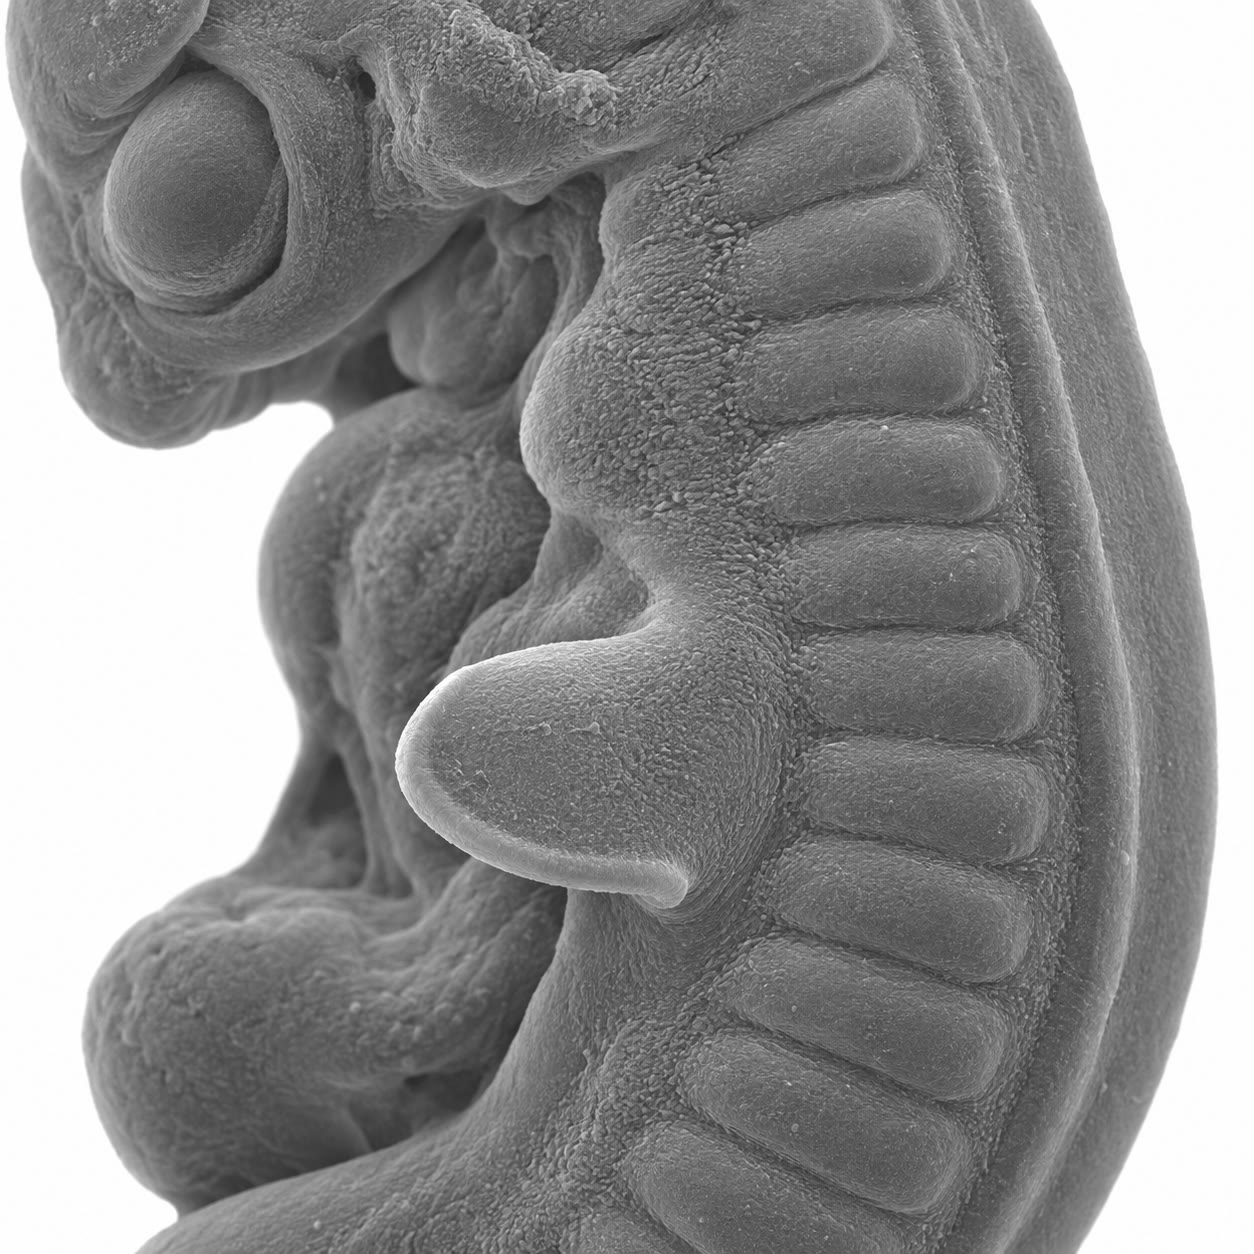
\includegraphics[width=0.42\linewidth]{images/book4/ai/b4-11-limb-bud.jpg}

{\small جنين كتكوت تحت المجهر الإلكتروني الماسح: صف
القُطَيعات على امتداد الجذع، وعلى الخاصرة \omterm{def:b2:limb-organogenesis:bud}{برعم الطرف}
المجدافي الشكل بعرفه المثخن على امتداد حافته.}
\end{omfigure}

\section{النمو الخارجي: المحور الداني--القاصي}

\begin{proposition}[العرف الأديمي القمي]\label{prop:b2:limb-organogenesis:aer}
\index{عامل نمو الأرومات الليفية}\index{منطقة التقدم}
العرف لازم للنمو الخارجي وعوامل FGF فيه كافية: فالأديم
المتوسط تحته، أي \emph{\omterm{prop:b2:limb-organogenesis:aer}{منطقة التقدم}}، ينقسم كل اثنتي عشرة
ساعة تقريبًا، والخلايا التي تغادر المنطقة مع تقدم القمة تكف
عن الانقسام وتتكثف وتتمايز. ويتكون الهيكل بالترتيب
الداني--القاصي --- \emph{القطعة الجذعية} (العضد أو الفخذ)،
و\emph{القطعة الوسطى} (الكعبرة والزند، والظنبوب والشظية)، و\emph{القطعة الطرفية}
(الرسغ والأصابع) --- ويُحدَّد كل مقطع بدوره مع نمو
البرعم، وتقابل المقاطعُ نطقًا متداخلة من التعبير عن مورّثات Hox
(وهي Hoxa/d 9--10 في القطعة الجذعية، و11 في الوسطى، و13 في
الطرفية). وينمو \omterm{def:b2:limb-organogenesis:bud}{برعم الطرف} نحو عشرة أضعاف في الطول في أربعة أيام
بينما يبقى مدى إشارة العرف بضع مئات من
الميكرومترات، فينمّط العرف الطرفَ لا دفعة واحدة بل
جبهةً متحركة، كما تضع طابعة صفحةً سطرًا سطرًا.
\end{proposition}
\begin{proof}[شواهد]
نزع سوندرز (1948) \omterm{def:b2:limb-organogenesis:bud}{العرف الأديمي القمي} من براعم أجنحة الكتاكيت في
أطوار متعاقبة: فحين نُزع باكرًا لم يعط البرعم إلا جذمورًا من العضد؛
وحين نُزع بعد يوم أعطى عضدًا وساعدًا بلا يد؛ وحين نُزع متأخرًا
أكثر أعطى جناحًا شبه كامل --- فكلما تأخرت العملية كان مستوى
البتر أقصى، إذن العرف لازم لكل مقطع بدوره. وأنتج
تطعيم عرف ثانٍ نموًا خارجيًا ثانيًا؛ وحبة مشبعة بعامل FGF،
موضوعة على برعم نُزع عرفه، أعادت طرفًا كاملًا (نيسواندر، 1993)، وحبة
موضوعة على الخاصرة بين حقلي الطرفين استحثت طرفًا زائدًا.
والفئران التي تفتقر إلى عوامل FGF العرفية بلا أطراف.
\end{proof}

\begin{omfigure}
\begin{tikzpicture}[every node/.style={font=\scriptsize}]
  \foreach \x/\lab/\n in {0/{العرف منزوع باكرًا:\\عضد فقط}/1, 3.6/{منزوع بعد يوم:\\عضد وكعبرة وزند}/2, 7.2/{منزوع متأخرًا أكثر:\\جناح شبه كامل}/3, 10.8/{سليم:\\جناح كامل}/4} {
    \begin{scope}[xshift=\x cm]
      \fill[omExo!25] (0,-0.5) rectangle (0.5,2.6);
      % humerus
      \draw[thick, fill=omDef!25, rounded corners=3pt] (0.6,0.9) rectangle (1.7,1.2);
      \ifnum\n>1 \draw[thick, fill=omDef!25, rounded corners=3pt] (1.8,1.05) rectangle (2.7,1.3); \draw[thick, fill=omDef!25, rounded corners=3pt] (1.8,0.75) rectangle (2.7,1.0); \fi
      \ifnum\n>2 \foreach \y in {0.55,0.85,1.15} \draw[thick, fill=omDef!25, rounded corners=2pt] (2.8,\y) rectangle (3.3,\y+0.2); \fi
      \ifnum\n=4 \foreach \y in {0.55,0.85,1.15} \draw[thick, fill=omDef!25, rounded corners=2pt] (3.35,\y) rectangle (3.5,\y+0.2); \fi
      \node[below, align=center] at (1.8,-0.2) {\lab};
    \end{scope}
  }
\end{tikzpicture}

{\small تجربة سوندرز. كلما نُزع العرف أبكر كان المفقود
من الطرف أكثر، ودائمًا من القمة: فالعرف لازم لكل مقطع
وهو يُوضع.}
\end{omfigure}

\begin{theorem}[النمو بالانقسام]\label{thm:b2:limb-organogenesis:growth}
البرعم الذي تنقسم خلاياه كل $T$ ساعة يضرب عدد خلاياه
في $2^{t/T}$ في زمن $t$؛ فأربعة أيام بدورات من اثنتي عشرة ساعة تعطي
$2^{8} = 256$. وإذا نما حجم البرعم ألف ضعف في تلك
الأيام الأربعة، وفّر الانقسام عامل 256 وكان على عامل
الأربعة الباقي أن يأتي من تضخم الخلايا ومن الحشوة
التي تفرزها خلايا الغضروف حولها. وعلى العكس، فالمقطع
الذي يستغرق تحديده دورة خلوية واحدة --- أي نحو اثنتي عشرة
ساعة تفصل بين مستويات البتر المتعاقبة في تجربة
سوندرز --- يقابل مضاعفة واحدة \omterm{prop:b2:limb-organogenesis:aer}{لمنطقة التقدم}.
\end{theorem}
\begin{proof}
$N(t) = N_0 2^{t/T}$؛ فمع $t = \qty{96}{h}$ و$T = \qty{12}{h}$،
يكون $t/T = 8$. ونسبة العامل المطلوب إلى عامل الانقسام،
$1000/256 \approx 4$، هي ما يجب أن يوفره النمو غير الانقسامي.
\end{proof}

\section{الأصابع: المحور الأمامي--الخلفي}

\begin{proposition}[منطقة النشاط المستقطب]\label{prop:b2:limb-organogenesis:zpa}
\index{Sonic hedgehog}\index{مورفوجين!Shh}
تحدد \omterm{def:b2:limb-organogenesis:bud}{منطقة النشاط المستقطب} أي إصبع يتكون وأين. فخلاياها تفرز
\omterm{prop:b2:limb-organogenesis:zpa}{Sonic hedgehog} الذي ينتشر عبر البرعم من الحافة الخلفية،
وتقرأ خلايا الأديم المتوسط التركيز --- والزمن الذي
تعرضت له --- موضعًا: فأعلى جرعة تعطي الإصبع
الأكثر خلفية، والجرع الأدنى تعطي الأصابع الأمامية، ودون
عتبة لا يتكون إصبع البتة. وللتدرج الشكل الأسّي الذي في
\cref{ch:b2:vertebrate-development}، بطول تناقص من بضع
عشرات من الميكرومترات، وتقطع عتباته البرعم إلى
بدائيات الأصابع: ففي جناح الكتكوت، من الخلف إلى
الأمام، الأصابع 4 و3 و2. ويعطي منبع ثانٍ للإشارة عند
الحافة الأمامية طقمًا ثانيًا في صورة مرآة؛ ويعطي منبع أضعف،
أو تعرض أقصر، الأصابع الأمامية وحدها من الطقم الزائد.
والمورّثة نفسها، في الدور نفسه، تنمّط أصابع كل رباعي أرجل،
\omterm{def:b2:genome-diversification:mutation}{والطفرة} التي تضيف منبعًا أماميًا لبروتين Shh تعطي تعدد الأصابع عند القطط
والدجاج والفئران والناس.
\end{proposition}
\begin{proof}[شواهد]
طعّم سوندرز وغاسيلينغ (1968) كتلة من أديم الحافة الخلفية المتوسط
من برعم جناح كتكوت إلى الحافة الأمامية لبرعم آخر:
فأنمى المضيف جناحًا بستة أصابع بالترتيب 4-3-2-2-3-4،
أي صورة مرآة حول الوسط. وبيّنت تيكل (1975) أن عدد
الأصابع الزائدة يتوقف على عدد الخلايا المطعّمة --- أي على جرعة.
ووجد ريدل وتابن (1993) أن النسيج المطعّم يعبّر عن
مورّثة \emph{\omterm{prop:b2:limb-organogenesis:zpa}{Sonic hedgehog}}، وأن المورّثة لا يُعبَّر عنها في مكان آخر
من البرعم، وأن خلايا هُندست لتعبّر عنها، مطعّمةً
أماميًا، أعادت إنتاج التضاعف المرآوي؛ وفعلت حبة من البروتين
الشيء نفسه. والطافرات من الدجاج التي فيها رقعة Shh أمامية شاذة
لها أصابع أمامية زائدة.
\end{proof}

\begin{omfigure}
\begin{tikzpicture}[every node/.style={font=\scriptsize}, >=stealth]
  % normal bud with gradient and digits
  \begin{scope}
    \fill[omExo!25] (0,-0.3) rectangle (0.4,3.3);
    \shade[bottom color=omProp!60, top color=white] (0.4,-0.3) rectangle (3.2,3.3);
    \draw[thick] (0.4,-0.3) rectangle (3.2,3.3);
    \draw[thick, omProp, fill=omProp!70] (0.9,0.1) ellipse (0.45 and 0.35); \node[omProp!80!black, anchor=west] at (1.4,0.1) {ZPA};
    \foreach \y/\d in {0.6/4, 1.5/3, 2.4/2} { \draw[thick, fill=omDef!25, rounded corners=2pt] (3.3,\y-0.12) rectangle (4.2,\y+0.12); \node[right] at (4.25,\y) {الإصبع \d}; }
    \node[below, align=center] at (2.0,-0.5) {برعم سليم: Shh من\\الحافة الخلفية، والأصابع 4-3-2};
    \draw[->, thick] (-0.4,0.2) -- (-0.4,3.0); \node[rotate=90] at (-0.7,1.6) {خلفي $\to$ أمامي};
  \end{scope}
  % grafted bud
  \begin{scope}[xshift=7cm]
    \fill[omExo!25] (0,-0.3) rectangle (0.4,3.3);
    \shade[bottom color=omProp!60, top color=white] (0.4,-0.3) rectangle (3.2,1.5);
    \shade[top color=omProp!60, bottom color=white] (0.4,1.5) rectangle (3.2,3.3);
    \draw[thick] (0.4,-0.3) rectangle (3.2,3.3);
    \draw[thick, omProp, fill=omProp!70] (0.9,0.1) ellipse (0.45 and 0.35);
    \draw[thick, omProp, fill=omProp!70] (0.9,2.9) ellipse (0.45 and 0.35); \node[omProp!80!black, anchor=west] at (1.4,2.9) {ZPA مطعّمة};
    \foreach \y/\d in {0.3/4, 0.8/3, 1.3/2, 1.7/2, 2.2/3, 2.7/4} { \draw[thick, fill=omDef!25, rounded corners=2pt] (3.3,\y-0.1) rectangle (4.2,\y+0.1); \node[right] at (4.25,\y) {\d}; }
    \node[below, align=center] at (2.0,-0.5) {ZPA مطعّمة أماميًا:\\تضاعف مرآوي 4-3-2-2-3-4};
  \end{scope}
\end{tikzpicture}

{\small المنطقة المستقطبة. على اليمين: ينتشر Shh من الحافة
الخلفية ويحدد تركيزه الهابط الأصابع 4 و3 و2.
وعلى اليسار: منطقة ثانية مطعّمة على الحافة الأمامية تصنع تدرجًا
ثانيًا وطقمًا من الأصابع في صورة مرآة.}
\end{omfigure}

\begin{theorem}[حدود الأصابع من التدرج]\label{thm:b2:limb-organogenesis:thresholds}
مع Shh بتركيز $c_0$ عند الحافة الخلفية وطول تناقص
$\lambda$، يقع حد إقليم إصبع عتبته $T_i$ عند
$x_i = \lambda\ln(c_0/T_i)$ من الحافة. فمع $\lambda = \qty{50}{\micro m}$ وعتبات $0.6$
و$0.25$ و$0.08$ من $c_0$ للأصابع 4 و3 و2، تكون الأقاليم
$0$--$26$ و$26$--$69$ و$69$--$126$ ميكرومترًا، ولا يكوّن
النسيج وراء \qty{126}{\micro m} إصبعًا. ومضاعفة المنبع
تحرك كل حد إلى الخارج بمقدار $\lambda\ln 2 = \qty{35}{\micro m}$
--- وهو ما يكفي، في برعم بضع مئات من الميكرومترات، لإضافة إصبع عند
الحافة الأمامية؛ ومنبع ثانٍ عند الحافة الأمامية يضع
الأقاليم نفسها بالمقلوب.
\end{theorem}
\begin{proof}
من $c(x) = c_0 e^{-x/\lambda}$، يكون $c = T_i$ عند $x_i = \lambda
\ln(c_0/T_i)$: أي $50\ln(1/0.6) = 25.5$، و$50\ln 4 = 69$، و$50\ln 12.5 =
126$. وتعويض $c_0$ بالمقدار $2c_0$ يضيف $\lambda\ln 2$ إلى كل $x_i$.
\end{proof}

\begin{omfigure}
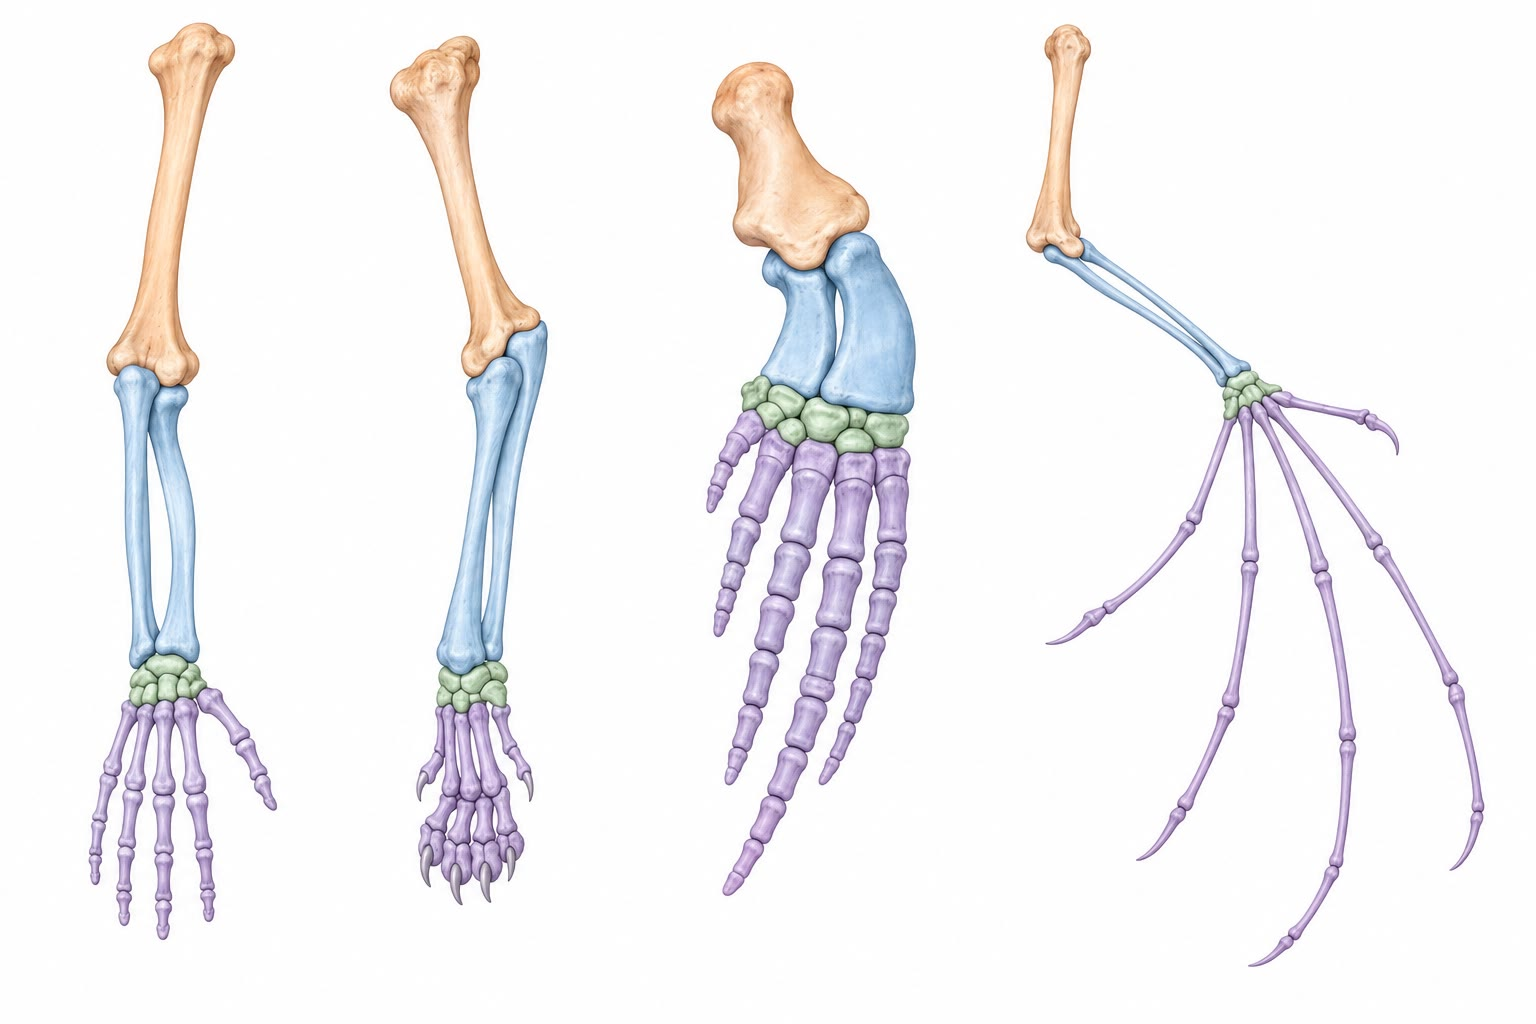
\includegraphics[width=0.66\linewidth]{images/book4/ai/b4-11-tetrapod-limbs.jpg}

{\small مخطط واحد، وأربعة أطراف: الأطراف الأمامية لإنسان وقط و
حوت وخفاش تتشارك العظام نفسها بالترتيب نفسه --- قطعة
جذعية واحدة، وعظمان في الوسطى، ورسغ، وأصابع --- مبنية بمراكز الإشارة
نفسها ومختلفة في النمو.}
\end{omfigure}

\section{التنسيق والنحت}

\begin{proposition}[المحاور يتحدث بعضها إلى بعض]\label{prop:b2:limb-organogenesis:loop}
\index{حلقة تغذية راجعة!نمائية}
تصون المراكز بعضها بعضًا: فعامل FGF من العرف يبقي \omterm{def:b2:limb-organogenesis:bud}{منطقة النشاط
المستقطب} معبّرة عن Shh، وShh، عبر مرحّل في الأديم المتوسط، يبقي
العرف معبّرًا عن FGF؛ وانزع أيهما يخفت الآخر في غضون
يوم. وWnt7a من الأديم الظاهر الظهري لازم للتعبير الكامل عن
Shh أيضًا، وهو يقود المصير الظهري للأديم المتوسط
(فالفأر الذي يفتقر إليه له راحتان). وهذا التعالق المتبادل
\emph{حلقة تغذية راجعة موجبة} تقفل المحاور الثلاثة معًا:
فلا ينمو الطرف إلا حيث يُنمَّط، ولا يُنمَّط
إلا حيث ينمو، فلا يصنع البرعم يدًا قط بلا
ذراع ولا أصابع من الصنف الخطأ. وحين يتم النمو الخارجي تُكسر
الحلقة --- فيكف الأديم المتوسط عن الترحيل، ويتوقف Shh، ويضمر
العرف --- ويتوقف الطرف عن النمو عند قياسه الصحيح.
\end{proposition}

\begin{proposition}[من النميط إلى العظم]\label{prop:b2:limb-organogenesis:skeleton}
\index{تكوّن الغضروف}\index{استماتة!بين الأصابع}
متى تحددت خلايا الأديم المتوسط المغادرة \omterm{prop:b2:limb-organogenesis:aer}{لمنطقة التقدم}
\emph{تكثفت} قضبانًا وصفائح بشكل العظام المقبلة، و
تمايزت إلى خلايا غضروفية تفرز حشوة غنية
بالكولاجين وعديدات السكريد البروتينية، ووضعت نموذجًا غضروفيًا لكل
عنصر هيكلي؛ وتتكون المفاصل حيث يُقال لشريط من الخلايا ألا
يصير غضروفًا؛ وتغزو الأوعية الدموية النماذج ويحل العظم محل
الغضروف من المركز إلى الخارج، تاركًا صفيحتي نمو عند
الطرفين تبقيان العظم يطول حتى البلوغ
(\emph{التعظم داخل الغضروف}). وتهاجر طلائع العضل من
القُطَيعات إلى الداخل، فتنقسم وتندمج أليافًا
(\cref{ch:b2:cell-differentiation}) وترتبط بأوتار يصنعها
الأديم المتوسط الخاص بالطرف. وبين أشعة الأصابع، يُزال النسيج
بموت خلوي مبرمج: فخلايا الأنسجة بين الإصبعية،
حين يقول لها بروتين مورفوجيني عظمي (BMP)، تفعّل
تدميرها الذاتي وتُزال في يوم، فتنفصل
الأصابع. والبطة تحتفظ بأغشيتها لأن مثبط BMP يُعبَّر عنه
في نسيجها بين الإصبعي؛ والكتكوت الذي يُعطى المثبط نفسه على
حبة تنمو له أقدام مكفَّفة.
\end{proposition}
\begin{proof}[شواهد]
الأديم المتوسط بين الإصبعي المقطوع من برعم رجل كتكوت والمطعّم
في مكان آخر يموت في موعده --- فالموت جوهري، مقرَّر
قبل نزع النسيج؛ والنسيج نفسه من بطة ينجو.
وحبات من BMP موضوعة بين أصابع بطة تميت الغشاء؛
وحبات من المثبط غريملين موضوعة بين أصابع كتكوت
تنقذه. والفأر الذي يفتقر إلى مستقبل BMP في الطرف يحتفظ بأغشيته.
\end{proof}

\begin{omfigure}
\begin{tikzpicture}[every node/.style={font=\scriptsize}]
  \foreach \x/\lab in {0/{أشعة الأصابع تتكثف\\غضروفًا}, 4.2/{الخلايا بين الإصبعية\\تموت (BMP)}, 8.4/{الأصابع منفصلة؛\\والعظم يحل محل الغضروف}} {
    \begin{scope}[xshift=\x cm]
      \node[below, align=center] at (1.5,-0.3) {\lab};
    \end{scope}
  }
  % stage 1: paddle with rays
  \draw[thick, fill=omDef!8] (0,0) .. controls (0,2.2) and (3,2.2) .. (3,0) -- cycle;
  \foreach \x in {0.6,1.2,1.8,2.4} \draw[thick, fill=omDef!30, rounded corners=2pt] (\x-0.12,0.1) rectangle (\x+0.12,1.5);
  % stage 2: paddle with dying webs
  \begin{scope}[xshift=4.2cm]
    \draw[thick, fill=omDef!8] (0,0) .. controls (0,2.2) and (3,2.2) .. (3,0) -- cycle;
    \foreach \x in {0.6,1.2,1.8,2.4} \draw[thick, fill=omDef!30, rounded corners=2pt] (\x-0.12,0.1) rectangle (\x+0.12,1.5);
    \foreach \x in {0.9,1.5,2.1} \foreach \y in {0.7,1.0,1.3} \fill[omThm] (\x,\y) circle (0.05);
  \end{scope}
  % stage 3: separated digits
  \begin{scope}[xshift=8.4cm]
    \draw[thick, fill=omDef!8] (0,0) -- (0,0.5) -- (0.3,0.5) -- (0.35,1.7) -- (0.85,1.7) -- (0.9,0.5) -- (1.05,0.5) -- (1.1,1.85) -- (1.6,1.85) -- (1.65,0.5) -- (1.8,0.5) -- (1.85,1.7) -- (2.35,1.7) -- (2.4,0.5) -- (2.7,0.5) -- (2.7,0) -- cycle;
    \foreach \x in {0.6,1.35,2.1} \draw[thick, fill=omExo!60, rounded corners=2pt] (\x-0.1,0.1) rectangle (\x+0.1,1.4);
  \end{scope}
\end{tikzpicture}

{\small نحت اليد: تتكثف أشعة الغضروف في المجداف،
وتموت الخلايا بينها (بالأحمر)، وتتعظم الأصابع المحرَّرة.}
\end{omfigure}

\begin{example}[الطرف نفسه، منمّى على نحو مختلف]\label{ex:b2:limb-organogenesis:evolution}
جناح الخفاش يد نمت أصابعها من 2 إلى 5 أطول بعدة
أضعاف من أصابع الفأر --- فمعزِّز لمورّثة طرفية، منقولًا
من الخفاش إلى الفأر، يطيل عظام الطرف الأمامي عند الفأر --- و
نجا نسيجها بين الإصبعي، لأن الغشاء يعبّر عن
مثبط BMP الذي تستعمله البطة. وزعنفة الحوت يد فيها
سلاميات زائدة وبلا موت بين إصبعي. ورجل الحصان
إصبع واحد اختُزل الباقي فيها إلى شظايا. والأفعى بلا
أطراف لأن خاصرتها لا تعبّر قط عن الإشارات التي تبدأ
البرعم. أما زعانف الأسماك، التي تفتقر إلى قطعة طرفية، فتُبنى
بالعرف وبمنطقة النشاط المستقطب نفسيهما لكنها توقف برنامج Hox قبل الطور المتأخر
الذي يصنع الأصابع؛ والأحفورة \emph{Tiktaalik} (وعمرها 375 مليون سنة)
تُظهر الرسغ وهو يظهر في زعنفة. فتطور الأطراف في جله
تعديل برنامج محفوظ --- أي كم يدوم كل طور، وإلى أين يبلغ
كل إشارة، وأي الخلايا تموت.
\end{example}

\section{تمارين}

\begin{exercise}[$\star$]\label{exo:b2:limb-organogenesis:1}
سمِّ محاور \omterm{def:b2:limb-organogenesis:bud}{برعم الطرف} الثلاثة، وسمِّ في كل منها مركز
الإشارة وموضعه وإشارته.
\end{exercise}

\begin{exercise}[$\star$]\label{exo:b2:limb-organogenesis:2}
أعط مقاطع هيكل الطرف الثلاثة وعظام كل منها
في ذراع الإنسان ورجله. وأي مورّثات Hox تعلّمها؟
\end{exercise}

\begin{exercise}[$\star$]\label{exo:b2:limb-organogenesis:3}
اذكر، بالترتيب، الخطوات من رقعة من أديم الصفيحة الجانبية المتوسط
إلى إصبع بعظمه ومفصله وعضلته.
\end{exercise}

\begin{exercise}[$\star$]\label{exo:b2:limb-organogenesis:4}
كيف يبدو الطرف إذا نُزع العرف (أ) حالما يظهر
البرعم، (ب) بعد تحديد الساعد، (ج) ولم يُنزع
البتة بل عُوّض بحبة من FGF؟
\end{exercise}

\begin{exercise}[$\star\star$]\label{exo:b2:limb-organogenesis:5}
مع $\lambda = \qty{40}{\micro m}$ وعتبات $0.5$ و$0.2$
و$0.05$ من تركيز المنبع للأصابع 4 و3 و2، احسب
الحدود الثلاثة وعرض إقليم كل إصبع.
\end{exercise}

\begin{exercise}[$\star\star$]\label{exo:b2:limb-organogenesis:6}
تنبّأ بنميط أصابع جناح كتكوت بعد (أ) منطقة نشاط مستقطب كاملة
مطعّمة على الحافة الأمامية، (ب) طُعم من ربع ذلك العدد من
خلايا المنطقة، (ج) حبة من Shh على الحافة الأمامية تُنزع بعد
تعرض قصير. اشرح كلًا منها بالجرعة والزمن.
\end{exercise}

\begin{exercise}[$\star\star$]\label{exo:b2:limb-organogenesis:7}
لبرعم طرف كتكوت \num{5000} خلية حين يتكون العرف وتنقسم
خلاياه كل \qty{12}{h}. فكم خلية بعد أربعة أيام؟ وإذا كان
للطرف في ذلك الطور $4\times 10^{6}$ خلية، فما الذي يجب أن يكون
صحيحًا في الدورة الخلوية أو في موت الخلايا؟
\end{exercise}

\begin{exercise}[$\star\star$]\label{exo:b2:limb-organogenesis:8}
اشرح لماذا يكون للكتكوت أصابع حرة وللبطة أقدام مكفَّفة، وماذا تفعل
حبة من مثبط BMP بين أصابع جنين كتكوت. وماذا
يقول لك التوقيت الجوهري للموت بين الإصبعي (فهو يقع في
موعده في طُعم) عن الطريقة التي عُلّمت بها الخلايا؟
\end{exercise}

\begin{exercise}[$\star\star$]\label{exo:b2:limb-organogenesis:9}
فأر يفتقر إلى Hoxa13 وHoxd13 معًا؛ وآخر يفتقر إلى Hoxa11 و
Hoxd11. تنبّأ بهيكل طرفه الأمامي في كل منهما وقل ماذا تبين
النتيجة عن العلاقة بين نطق Hox والمقاطع.
\end{exercise}

\begin{exercise}[$\star\star\star$]\label{exo:b2:limb-organogenesis:10}
اشرح التغذية الراجعة الموجبة بين العرف \omterm{def:b2:limb-organogenesis:bud}{ومنطقة النشاط المستقطب}، ولماذا
تجعل الطرف متينًا، وماذا كان ليحدث لبرعم لا يستطيع Shh فيه
أن يصون FGF. وقابل ذلك بالتغذية الراجعة الموجبة في
المخاض في \cref{ch:b2:mammal-reproduction}: ما الذي ينهي كل حلقة؟
\end{exercise}

\begin{exercise}[$\star\star\star$]\label{exo:b2:limb-organogenesis:11}
إصبع الخفاش الثالث أطول ثماني مرات من إصبع الفأر نسبةً
إلى قياس الجسم. فإذا طال غضروف الإصبع أسّيًا بمعدل
$r$ في اليوم خلال نافذة نمو، وكانت نافذة الخفاش أطول بأربعة
أيام من نافذة الفأر، فأي $r$ يلزم؟ أعط تغيرين
نمائيين (أحدهما في النمو والآخر في موت الخلايا) يصنعان
جناحًا من يد.
\end{exercise}

\begin{exercise}[$\star\star\star$]\label{exo:b2:limb-organogenesis:12}
ينمّط \omterm{prop:b2:limb-organogenesis:zpa}{Sonic hedgehog} \omterm{prop:b2:vertebrate-development:neurulation}{الأنبوب العصبي} من صفيحة الأرض
(\cref{ch:b2:vertebrate-development}) والأصابع من \omterm{def:b2:limb-organogenesis:bud}{منطقة النشاط المستقطب}.
ناقش لماذا يعيد التطور استعمال إشارات قليلة لأعمال كثيرة، وكيف
يمكن للجزيئة نفسها أن تعني أشياء مختلفة في أنسجة مختلفة، وماذا
يعني هذا في أثر \omterm{def:b2:genome-diversification:mutation}{طفرة} في مورّثة كهذه.
\end{exercise}

\section{مسألة: جناح يُبنى في أسبوع}

\begin{problem}[{مسألة نهاية الأسبوع --- متابعة جناح الكتكوت من البرعم
إلى الهيكل: نموه بالانقسام، وتوقيت نزوعات العرف عند سوندرز،
وحساب تدرج Shh والتنبؤ بتضاعفاته، ونحت الأغشية ومقارنة الجناح
بجناح خفاش، وتنتهي إلى عدد المضاعفات وحدود الأصابع والعرض الذي
يحتاجه البرعم لتضاعف مرآوي}]
\label{pb:b2:limb-organogenesis:1}
يظهر برعم جناح الكتكوت عند 3 أيام من الحضن وله \num{2000}
خلية أديم متوسط وطول \qty{0.4}{mm}؛ وعند 7 أيام يكون الجناح
بطول \qty{4}{mm} وحجمه \num{1000} ضعف حجم البرعم. وخلايا \omterm{prop:b2:limb-organogenesis:aer}{منطقة
التقدم} تنقسم كل \qty{12}{h}. ونزوعات العرف: عند 3.0 أيام يكون
الطرف جذمورًا؛ وعند 3.5 أيام عضدًا فقط؛ وعند 4.0 أيام عضدًا
وكعبرة وزندًا؛ وعند 4.5 أيام جناحًا ينقصه أطراف الأصابع فقط.
وShh: $D = \qty{1e-12}{m^2/s}$، وعمر نصف \qty{29}{min}؛ والعتبات
$0.6$ و$0.25$ و$0.08$ من $c_0$ للأصابع 4 و3 و2. وعرض البرعم (من الخلف
إلى الأمام) \qty{600}{\micro m}. والأغشية بين الإصبعية: ثلاث مناطق
قياس كل منها \qty{300}{\micro m}$\times$\qty{300}{\micro m}$\times$\qty{200}{\micro m}، وخلاياها
بحجم \qty{1000}{\micro m^3}، تُزال في \qty{24}{h}.

\medskip
\noindent\textbf{الجزء الأول --- النمو.}
\begin{enumerate}
  \item كم مضاعفة تقع في أربعة أيام؟ وكم خلية تعطي
        انطلاقًا من \num{2000}؟
  \item قارن ذلك بازدياد الحجم ألف ضعف: فأي عامل
        يجب أن يوفره تضخم الخلايا والحشوة؟
  \item بأي عامل نما الطول؟ وإذا نما البرعم أسطوانةً
        ثابتة نصف القطر، فأي عامل حجم كان ليعطي، وماذا
        يقول الفرق عن الشكل؟
  \item يبلغ عامل FGF العرفي \qty{300}{\micro m} داخل الأديم المتوسط.
        فما كسر البرعم الواقع تحت تأثيره عند 3 أيام
        وعند 7 أيام؟
  \item اشرح لماذا تنتج إشارة ثابتة المدى في عضو نامٍ
        تعاقبًا دانيًا--قاصيًا.
  \item خلية تغادر \omterm{prop:b2:limb-organogenesis:aer}{منطقة التقدم} عند 4 أيام. فأي مقطع
        تنضم إليه؟
\end{enumerate}

\medskip
\noindent\textbf{الجزء الثاني --- توقيت المقاطع.}
\begin{enumerate}[resume]
  \item من سلسلة النزوعات، أعط الزمن الذي يكون قد تحدد عنده كل
        مقطع (القطعة الجذعية، والوسطى، والطرفية).
  \item كم دورة خلوية تفصل بين تحديد
        المقاطع المتعاقبة؟
  \item اشرح النتيجة بدلالة \omterm{prop:b2:limb-organogenesis:aer}{منطقة التقدم} و
        نطق Hox.
  \item توضع حبة FGF على برعم نُزع عرفه عند 3.5
        أيام. تنبّأ بالطرف.
  \item يُطعَّم عرف ثانٍ على السطح الظهري لبرعم
        سليم عند 3.5 أيام. تنبّأ.
  \item لماذا يكف البرعم عن النمو عند 7 أيام بدل أن
        يستمر بلا نهاية؟
\end{enumerate}

\medskip
\noindent\textbf{الجزء الثالث --- التدرج.}
\begin{enumerate}[resume]
  \item احسب $k$ و$\lambda$ من أجل Shh.
  \item احسب حدود الأصابع الثلاثة وعروض الأقاليم.
  \item كم يبلغ عرض المنطقة الأمامية التي لا تكوّن إصبعًا في
        برعم عرضه \qty{600}{\micro m}؟
  \item \omterm{def:b2:genome-diversification:mutation}{طفرة} تضاعف خرج Shh. أعد حساب الحدود و
        قل هل يتكون إصبع زائد وأيها.
  \item تُطعَّم منطقة نشاط مستقطب على الحافة الأمامية. فما أدنى عرض
        للبرعم يتيح طقمًا مرآويًا كاملًا 4-3-2-2-3-4 دون
        تداخل إقليمي الإصبع 2؟ وهل برعم الكتكوت عريض
        بما يكفي؟
  \item تنبّأ بالنميط لو كان عرض البرعم \qty{200}{\micro m}
        فقط.
  \item لماذا يعطي طُعم من ربع \omterm{def:b2:limb-organogenesis:bud}{منطقة النشاط المستقطب} النميط 2-2-3-4 فقط؟
\end{enumerate}

\medskip
\noindent\textbf{الجزء الرابع --- النحت والتطور.}
\begin{enumerate}[resume]
  \item احسب عدد الخلايا في الأغشية الثلاثة ومعدل
        موت الخلايا خلال الإزالة، بالخلايا في الثانية.
  \item تعبّر خلايا البطة بين الإصبعية عن مثبط BMP. تنبّأ
        بأثر حبة من BMP في غشاء بطة وبأثر
        المثبط في غشاء كتكوت.
  \item ينمو غضروف إصبع الخفاش أربعة أيام زائدة بمعدل
        أسّي قدره \qty{0.5}{d^{-1}}. فبأي عامل يكون
        أطول من إصبع الكتكوت؟ وسمِّ تغيرًا ثانيًا يصنع
        غشاء الجناح.
  \item لبرعم زعنفة سمكة عرف ومنطقة نشاط مستقطب لكن بلا أصابع. فما
        المفقود، وماذا تُظهر \emph{Tiktaalik}؟
  \item لو أُنتجت خلايا الأغشية بدل ذلك بالانقسام من
        \num{1000} مؤسِّس عند \qty{12}{h} للدورة، فكم كان
        صنعها ليستغرق؟ وقارن ذلك باليوم الذي تستغرقه
        إزالتها.
  \item اذكر النتيجة: المضاعفات في أربعة أيام، وحدود الأصابع
        الثلاثة، وأدنى عرض لتضاعف مرآوي.
\end{enumerate}
\end{problem}
